\documentclass[10pt]{beamer}

\usetheme[progressbar=frametitle]{metropolis}
\usepackage{appendixnumberbeamer}

\usepackage{booktabs}
\usepackage[scale=2]{ccicons}

\usepackage{tabulary}
\usepackage[normalem]{ulem}

\usepackage{pgfplots}
\usepgfplotslibrary{dateplot}

\usepackage{xspace}
\newcommand{\themename}{\textbf{\textsc{metropolis}}\xspace}

\title{Detecção de artefatos de arritmia utilizando Máquinas de Vetores de Suporte e Coeficientes de Energia Wavelet}
\subtitle{Proposta de TCC}
% \date{\today}
\date{2020}
\author{Gabriel Lechenco Vargas Pereira \\
Cristiano Marcos Agulhari}
\institute{Universidade Tecnológica Federal do Paraná - UTFPR}
% \titlegraphic{\hfill\includegraphics[height=1.5cm]{logo.pdf}} 

\begin{document}
\setbeamertemplate{frame footer}{Universidade Tecnológica Federal do Paraná}

\maketitle

\begin{frame}{Sumário}
  \setbeamertemplate{section in toc}[sections numbered]
  \tableofcontents[hideallsubsections]
\end{frame}

\section{Introdução}

\begin{frame}{Introdução}
    Doenças cardiovasculares
    \begin{itemize}
        \item Foram responsáveis por um terço das mortes em 2016
        \item Três quartos dessas ocorreram em países de baixa e média renda
        \item A principal causa das mortes são diagnóstico feito tardiamente
    \end{itemize}
\end{frame}

\begin{frame} {Justificativa}
  O desenvolvimento de modelos computacionais com a capacidade de identificar 
  artefatos de arritmia podem auxiliar em um diagnóstico mais rápido de doenças 
  cardiovasculares.
\end{frame}

\begin{frame}{Objetivo}

  

\end{frame}

\section{Fundamentação Teórica}

\begin{frame}{Eletrocardiograma}
    \begin{figure}[]
      \centering
      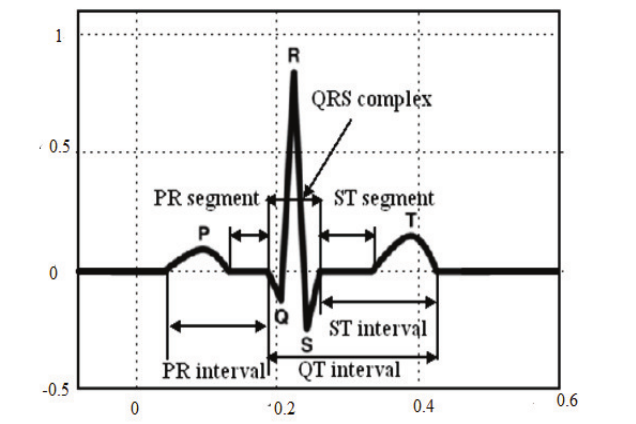
\includegraphics[width=8cm]{images/pqrst.png}
      \caption{Ciclo PQRST \cite{faziludeen_ecg_2013}}
      \label{fig:pqrst}
    \end{figure}
\end{frame}

\begin{frame}{Arritmia}
  A falta de ritmo cardíaco tem ampla influência sobre a saúde do paciente.
  \only<1>{
    \begin{itemize}
      \item Deficiência no transporte e fornecimento de oxigênio.
      \item Podendo acarretar complicações em todo o corpo.
      \item Algumas capazes de levar ao óbito em poucos minutos.
    \end{itemize}
  }

  % \only<2>{Imagem taquicardia ventricular}
  
  % \only<3>{Imagem fibrilação ventricular}
\end{frame}

\begin{frame}{Exemplo Eletrocardiograma}
  \only<1>{
    \begin{figure}
      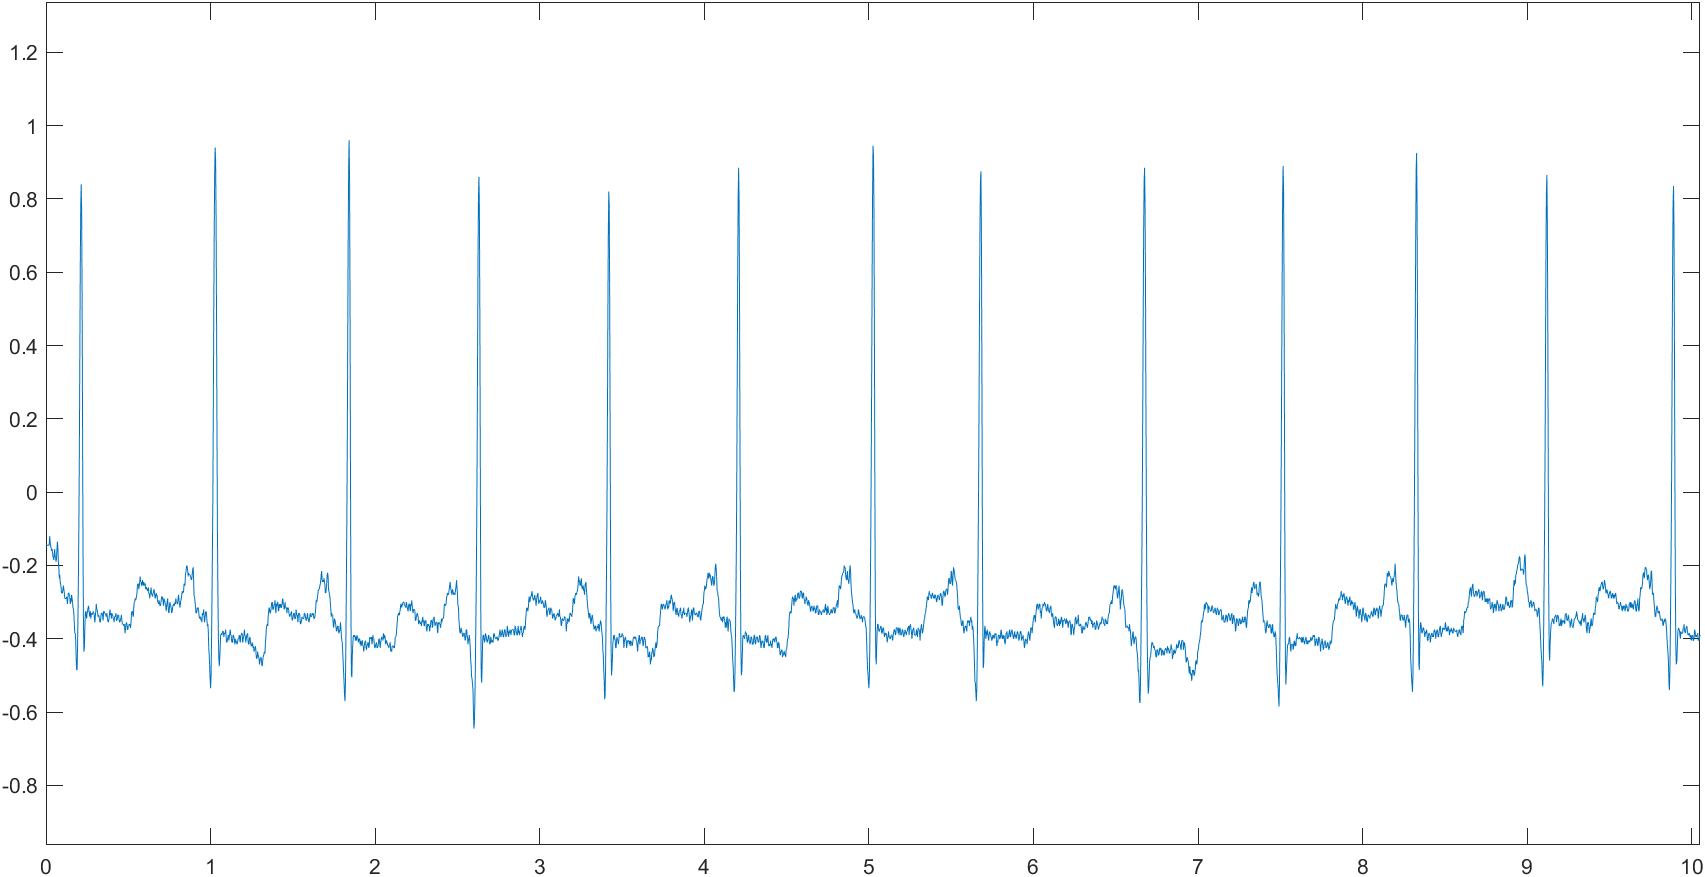
\includegraphics[width=10.5cm]{images/normal.png}
      \caption{Trecho batimentos ritmo normal}
    \end{figure}
  }
  
  \only<2>{
    \begin{figure}
      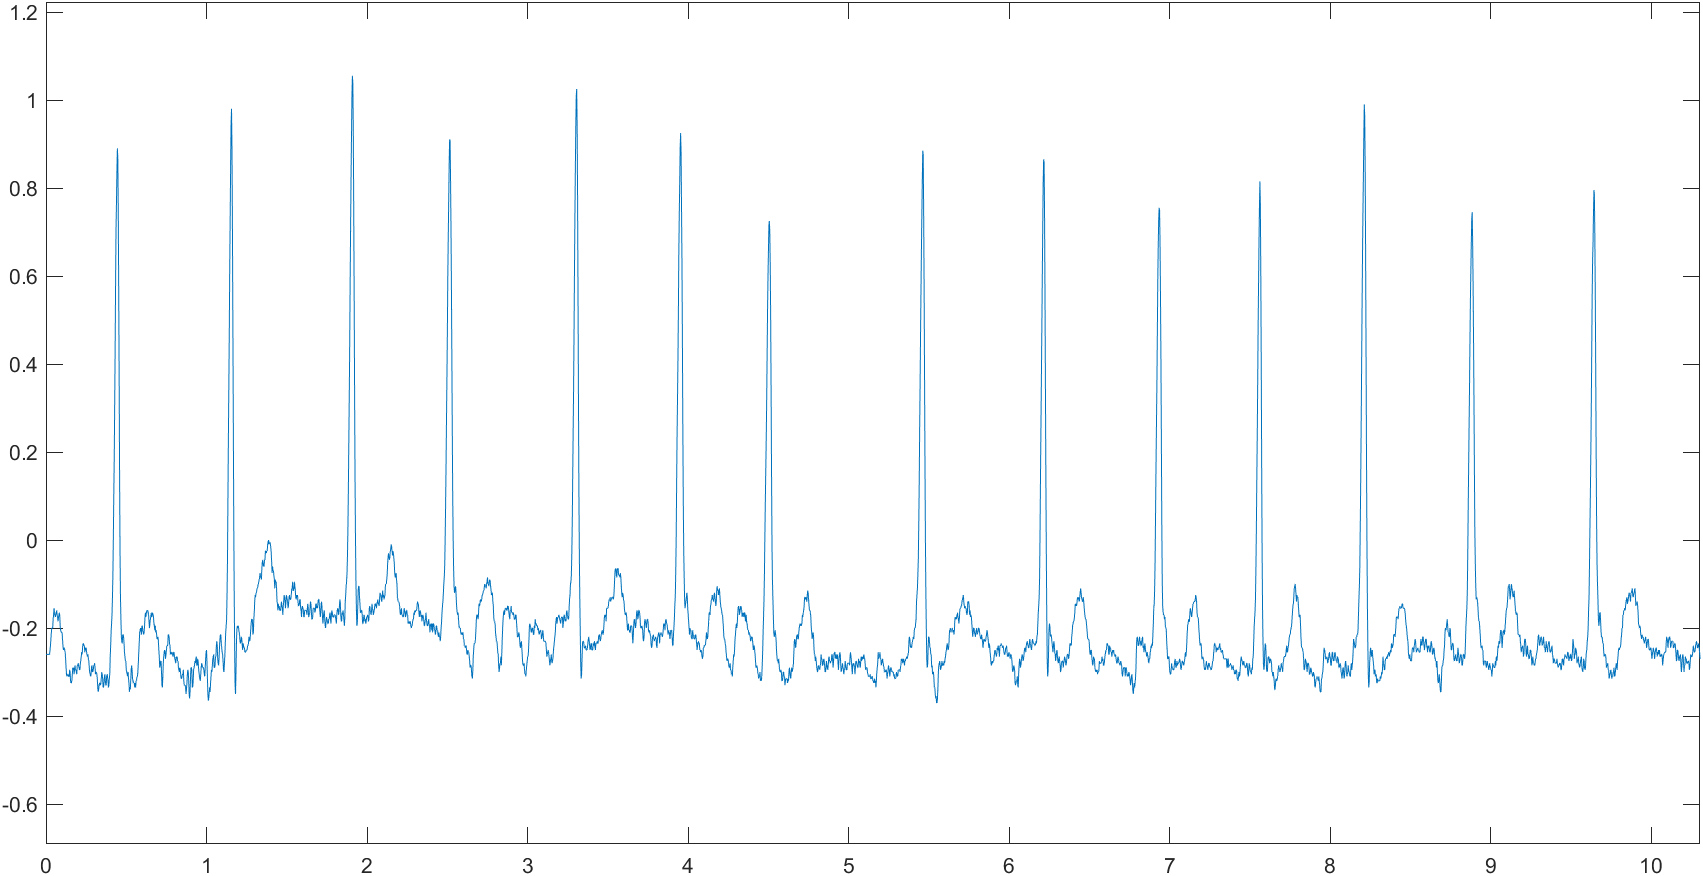
\includegraphics[width=10.5cm]{images/artrial_fibri.png}
      \caption{Trecho batimentos com fibrilação atrial}
    \end{figure}
  }

\end{frame}

\begin{frame}{Máquinas de Vetores de Suporte (SVM)}
    \only<1>{
      Algoritmo de classificação binária que busca encontrar o hiperplano 
      ótimo que seccione o hiperespaço onde os dados se encontram.

      \begin{equation}
        f(x) = \langle w, x \rangle + b = 0
        \nonumber
      \end{equation}

    }
    \only<2>{ 
      \begin{figure}[]
        \centering
        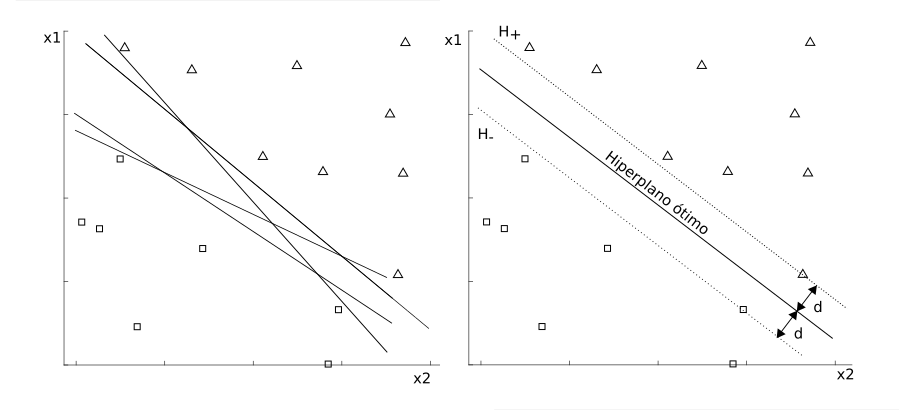
\includegraphics[width=10cm]{images/svmSample.png}
        \caption{Separação de dois planos por um hiperplano ótimo}
        \label{fig:svm}
      \end{figure}
    }
\end{frame}

\begin{frame}{Máquinas de Vetores de Suporte (SVM)}
  Vantagens 
  \begin{itemize}
    \item Otimização de natureza convexa
    \item Apresenta um unico mínimo global para problemas lineares
    \item Consegue bons resultados com poucos exemplos
  \end{itemize}

  \visible<2>{
    Desvantagens
    \begin{itemize}
      \item A princípio resolve apenas problemas lineares
      \item Classificação binária
    \end{itemize}
  }
\end{frame}

\begin{frame}{SVM's e problemas não lineares}
    \textbf{Teorema de Cover}
    \begin{quote}
      Dado um problema de classificação de padrões complexo, ao lançá-lo em 
      um espaço com muitas dimensões é mais provável que este seja linearmente 
      separável do que em um espaço com poucas dimensões, desde que o espaço não seja densamente preenchido.
      \cite{haykin_neural_2010}
    \end{quote}
\end{frame}

\begin{frame} {SVM's e problemas não lineares}
  A adição de diferentes kernels possibilita uma maior flexibilidade do algoritmo de
  SVM com uma pequena modificação no problema de otimização.
  \begin{equation}
    f(x) = \langle w, \psi(x) \rangle + b = 0
    \nonumber
  \end{equation}
\end{frame}

\begin{frame}{Problema XOR}
  \begin{figure}
    \centering
    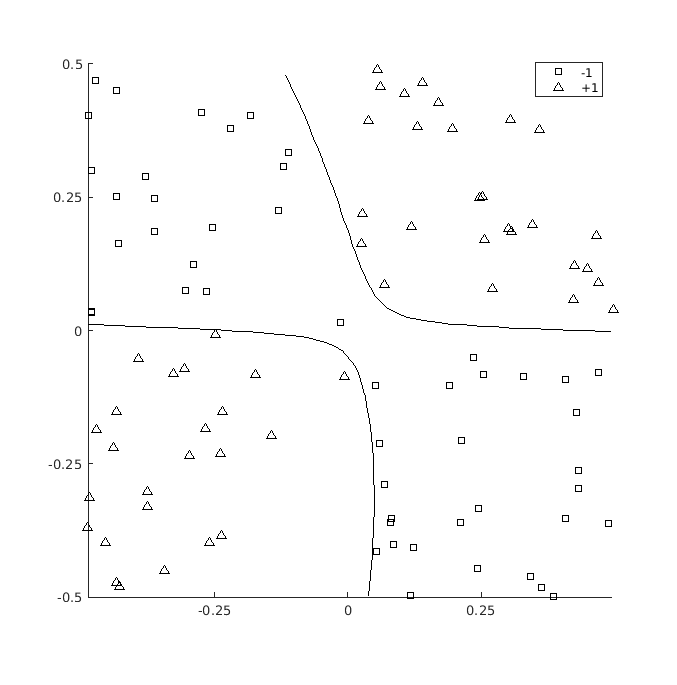
\includegraphics[width=6cm]{images/svmXor.png}
    \caption{SVM utilizando o kernel gaussiano para o problema XOR}
  \end{figure}
\end{frame}

\begin{frame}{SVM's e problemas não binários}

  \only<1>{
    Técnicas pra classificação não binária
    \begin{itemize}
      \item \textit{One Against All} (OAA)
      \item \textit{One Against One} (OAO)
      \item \textit{Directed Acyclic Graph SVM} (DAGSVM)
      \item \textit{Binary Tree of SVM} (BTS)
    \end{itemize}
  }

  \only<2>{\textit{Directed Acyclic Graph SVM} (DAGSVM)
    \begin{figure}[]
      \centering
      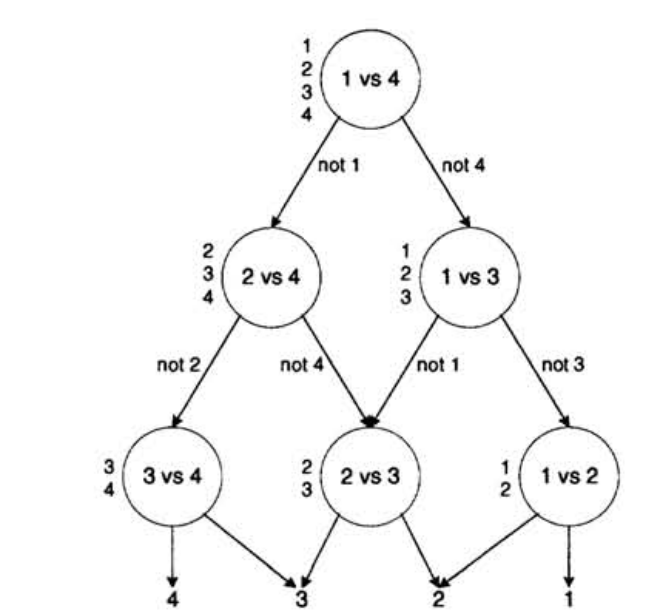
\includegraphics[width=6cm]{images/dagSVM.png}
    \end{figure}
  }
  \only<3>{\textit{Binary Tree of SVM} (BTS)
    \begin{figure}[]
      \centering
      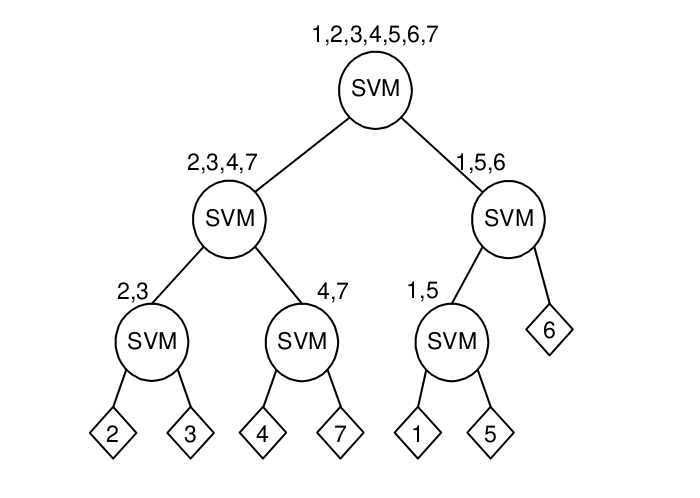
\includegraphics[width=7cm]{images/btsSample.png}
    \end{figure}
  }

\end{frame}

\begin{frame}{Wavelets}
    A Transformada de Fourier é amplamente utilizada no processamento de sinais digitais, 
    porém, ela pode não ser a mais adequada em alguns casos.

    Transformadas wavelet são mais apropriadas para a análise de fenômenos não 
    estacionários ou variantes no tempo.
\end{frame}

\begin{frame} {Wavelets}
  \begin{figure}[]
    \centering
    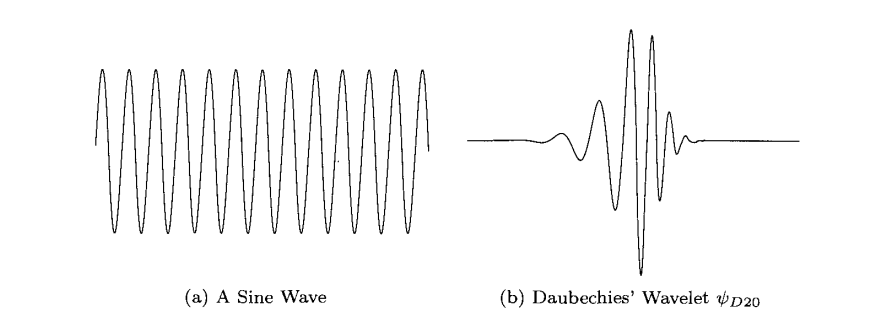
\includegraphics[width=10cm]{images/waveAndWavelet.png}
    \caption{Onda de energia e infinita e wavelet de energia concentrada}
  \end{figure}
\end{frame}

\begin{frame} {Wavelets}
  Características das funções Wavelet:
  \begin{itemize}
    \item Infinitas funções wavelet disponíveis
    \item Localização em tempo-frequência (Escala e Translação)
    \item Multirresolução
  \end{itemize}
\end{frame}


\begin{frame}{Multirresolução}

  % \begin{figure}[]
  %   \centering
  %   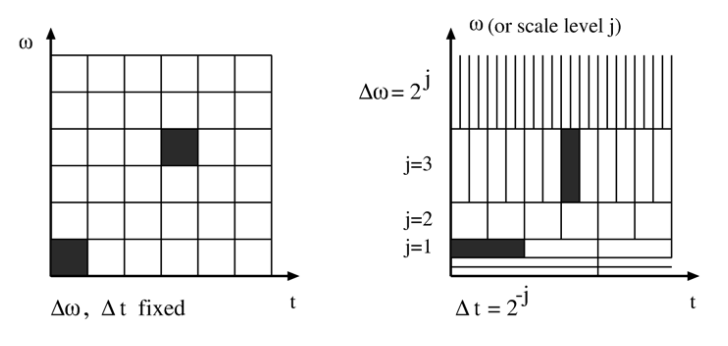
\includegraphics[width=10cm]{images/multiresolution.png}
  %   \caption{Resolução no tempo-frequência STFT e Decomposição Wavelet}
  % \end{figure}

\end{frame}

\begin{frame}{\textit{Filter Bank} e \textit{Wavelet Packets}}

  \only<1> {
    Ao tentar otimizar a propriedade de multirresolução, os \textit{Filter Banks}
    combinam as decomposições multiníveis em uma árvore binária, construindo 
    uma coleção de filtros passa-baixa e passa-alta.

    Enquanto que as \textit{Wavelet Packets} procuram uma análise mais completa 
    dos filtros, a partir de uma decomposição binária.
  }

  \only<2> {
    \begin{figure}[]
      \centering
      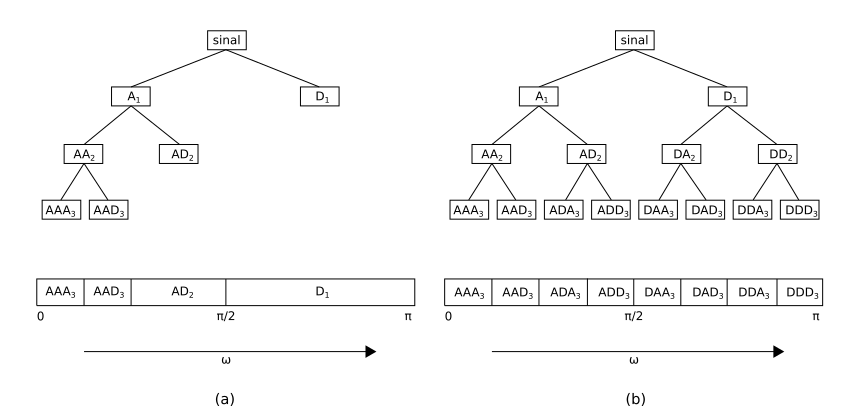
\includegraphics[width=10cm]{images/filterBankPacket.png}
      \caption{Árvores de Decomposição Wavelet}
    \end{figure}
  }

\end{frame}

\section{Revisão de Literatura}

\begin{frame}{Trabalhos Relacionados}

  \only<1>{
    \begin{table}
      \begin{tabulary}{\textwidth}{|C|C|}
          \hline
          Trabalho                               & Técnica   \\ \hline
          Govindan, Deng e Power (1997)  & Wavelet + Redes Neurais                                                      \\ \hline
          Zhao e Zhang (2005)        & Wavelet + SVM  + Modelagem Autorregressiva     \\ \hline
          Mora e Amaya (2012)         & Entropia de Shannon + Complexidade de Lempel-Ziv + SVM-OAO assimétrica   \\ \hline
          Rua et al. (2012)           & Energia Wavelet + Redes Neurais                                                                                      \\ \hline
          Azariadi et al. (2016)          & Wavelet +   SVM            \\ \hline
          Tuncer et al. (2019)      & Wavelet +  Localização de padrões  locais hexadecimais +  KNN  \\ \hline
      \end{tabulary}
    \end{table}
  }

  \only<2>{
    \begin{tabulary}{\textwidth}{|C|c|c|c|}
      \hline
      Trabalho                                                                          & Nº de classes & \begin{tabular}[c]{@{}l@{}}Nº de Exemplos \\no treinamento \end{tabular} & Acurácia       \\ \hline
      Govindan, Deng e Power (1997)                                            & $4$                                                            &                      $10$                            & $77\% \pm 9\%$ \\ \hline
      Zhao e Zhang (2005)                                                  & $6$                                                           &                 $7940$                                & $99,68\%$      \\ \hline
      Mora e Amaya (2012)                                                   & $5$                                                            &                $637$                                 & $90,72\%$      \\ \hline
      Rua et al. (2012)                                                     & $2$                                                           &               -                               & $99.46\%$      \\ \hline
      Azariadi et al. (2016)                                                    & $2$                                                           &                      104581                         & $97\%$         \\ \hline
      Tuncer et al. (2019)                                                & $17$                                                        &                        -                        & $95.0\%$       \\ \hline
  \end{tabulary}
  }

\end{frame}

\section{Proposta}

\begin{frame}{Proposta}
  \begin{figure}[]
    \centering
    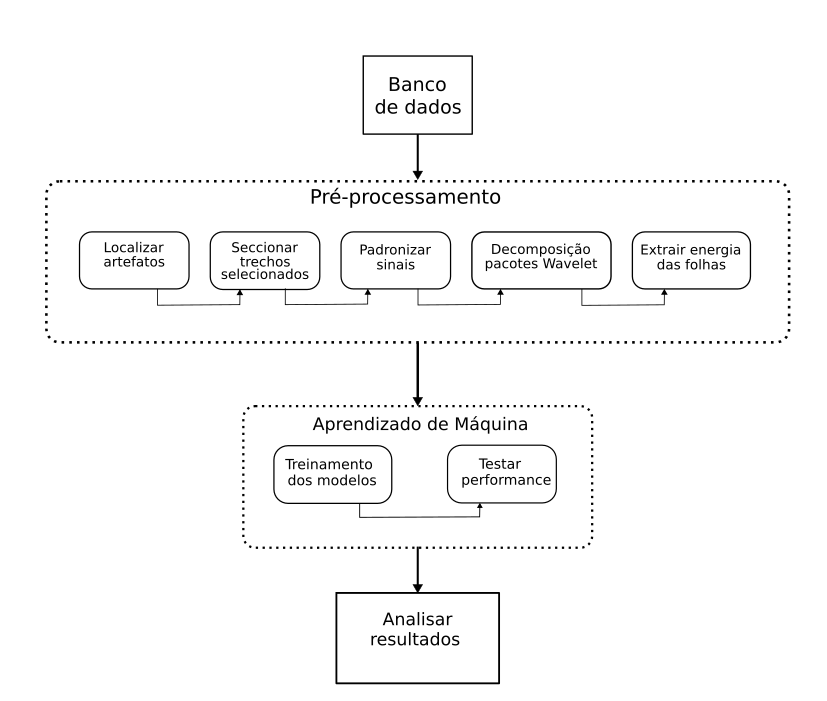
\includegraphics[height=6cm]{images/proposal.png}
    \caption{Descrição do Método que será utilizado}
  \end{figure}
\end{frame}

\begin{frame}{Bases de Dados}
  Bases de dados
  \begin{itemize}
    \item MIT-BIH Arrhythmia Database (mitdb)
    \only<2>{
      \begin{itemize}
        \item Trechos de arritmia
        \item Trechos saudáveis 
      \end{itemize}
    }
    \item MIT-BIH Normal Sinus Rhythm Database (nsrdb)
    \only<2>{
      \begin{itemize}
        \item Trechos saudáveis
      \end{itemize}
  }  \end{itemize}
\end{frame}

\begin{frame}{Pré-processamento}
  Localizar e seccionar trechos selecionados:
  \begin{itemize}
    \item Ler anotações e comentários presentes nas bases de dados
    \item Localizar o início e término de eventos arrítmicos
    \item Seccionar trechos a cada 8 segundos
    \alert<2>{\item Padronizar taxa de amostragem para $128 Hz$}
    \item Fazer o mesmo para os dados saudáveis
  \end{itemize}
\end{frame}

\begin{frame}{Extração de características}
  \only<1>{
    Cada trecho de sinal será decomposto até o quarto nível, no final a folha 
    mais a esquerda será decomposta por mais dois níveis. Será utilizada a 
    função \textit{Daubechies} com suporte 3, por se adequar bem aos sinais cardíacos.
  }
  \only<2> {
    \begin{figure}[]
      \centering
      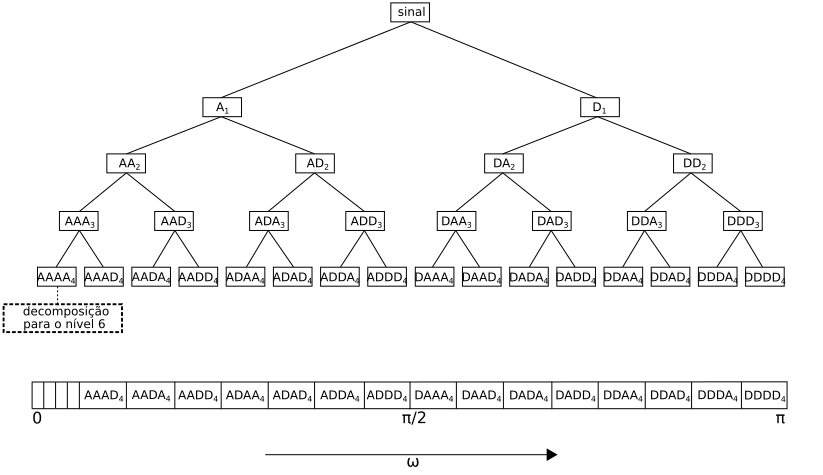
\includegraphics[width=10.5cm]{images/waveletProposal.png}
      \caption{Decomposição Wavelet proposta}
    \end{figure}
  }
\end{frame}

\begin{frame}{Aprendizado de Máquina}
  \only<1> {
    Máquinas de Vetores de Suporte (SVM)
    \begin{itemize}
      \item Aprendizado supervisionado
      \item Classificação entre 4 classes
      \item Comparação entre técnicas de classificação multiclasses
    \end{itemize}
  }

  \only<2>{
    Classificação entre 4 classes
    \begin{table}
      \centering
    \begin{tabular}{|c|c|}
      \hline
      Sigla   & Classe                        \\ \hline
      N       & Batimentos com ritmos normais \\ \hline
      AFIB    & Fibrilação Arterial           \\ \hline
      SBR     & Bradicardia Sinusal           \\ \hline
      ASV     & Arritmia Supraventricular     \\ \hline

    \end{tabular}
  \end{table}
  }
\end{frame}

% \begin{frame}{Testes e resultados}
    
% \end{frame}

\begin{frame}{Cronograma}
  \only<1>{
    \begin{tabulary}{\textwidth}{|l|C|}
      \hline
      Data        & Atividade                                                                                    \\ \hline
      14/Agosto   & Selecionar trechos relevantes dos sinais biológicos com base nas anotações do banco de dados \\ \hline
      28/Agosto   & Realizar o janelamento e padronização destes trechos                                         \\ \hline
      11/Setembro & Extrair Energias Wavelet                                                                     \\ \hline
      02/Outubro  & Realizar Classificações                                                                      \\ \hline
      23/Outubro  & Agrupar Resultados                                                                           \\ \hline
      20/Novembro & Descrever Resultados e Conclusões finais                                                     \\ \hline
      \end{tabulary}
  }
  \only<2>{
    \begin{tabulary}{\textwidth}{|l|C|}
      \hline
      Data        & Atividade                                                                                    \\ \hline
      14/Agosto   & \sout{Selecionar trechos relevantes dos sinais biológicos com base nas anotações do banco de dados} \\ \hline
      28/Agosto   & \sout{Realizar o janelamento e padronização destes trechos                                        } \\ \hline
      11/Setembro & \sout{ Extrair Energias Wavelet                                                                   } \\ \hline
      02/Outubro  & Realizar Classificações                                                                      \\ \hline
      23/Outubro  & Agrupar Resultados                                                                           \\ \hline
      20/Novembro & Descrever Resultados e Conclusões finais                                                     \\ \hline
      \end{tabulary}
  }
\end{frame}

\section{Considerações Finais}

% {\setbeamercolor{palette primary}{fg=white, bg=mDarkTeal}
% \begin{frame}[standout]
%   Perguntas?
% \end{frame}
% }

\appendix


\begin{frame}[allowframebreaks]{References}

  \bibliography{demo}
  \bibliographystyle{abbrv}

\end{frame}

\end{document}
